\chapter{Reduced precision}
\label{ch:reduced-precision}
Traditionally, computing application are developed to give exact results.
While this is necessary in certains fields (e.g. aerospace), results with a lower
precision is acceptable for multiple types of data.
As~\cite{Cherubin2020-tt} depicts, numerous studies explored the use of lower 
precision data type to perform computation.
It is an interesting strategy as it has the joint potential to reduce hardware 
size, energy cost, and execution time.
In this chapter, we explore (1) the problem definition of \textit{Reduced Precision},
(2) various data formats used to perform reduced precision,
(3) methods to implement reduced precision,
(4) the growth of quantization in Deep Learning,
and (5) discuss the benefits, limitation, and open questions of reduced precision.

\section{Problem definition}
\label{sc:rp-problem-definiton}
The IEEE~754 standard defines two main floating-point formats.
Altough although offering enough precision for most applications, it can also be unecessary precision.
That is, multiple type of application do not benefit from that much precision.
For this reason, a lot of efforts in creating new data formats with lower precision (discussed in~\ref{sc:rp-data-format}).
The idea behind reduced precision is to represent numbers in a data format with 
lower bit witdh; i.e. lower exponent or mantissa.
Similar mixed-precision is a concept that use data formats of different precision within a program allowing better tunning of data format.
The logic complexity of floating points is approximately proportional to the square of the bit width~\cite{Chen2018-an}.
Therefore, lowering the number of bit in a data format also reduce the dye size 
of a chip and, by consequence, the energy cost and computation time for arithmetic operations.

The work done in~\cite{Cherubin2020-tt} surveys a range of tools in the fields of reduced precision.
That same study define five challenges that remain to be addressed for reduced precision:
\begin{itemize}
	\item[1.] Identify the code sections where applying reduced precision is beneficial.
	\item[2.] Determine the data type to use base on the application and architecture.
	\item[3.] Estimate, quantify bounds and manage the numerical error introduced by applying reduced precision to an application.
	\item[4.] Measure the overhead from type casting between different data types.
	\item[5.] Develop a tool that benefit a wide range of applications and platforms.
\end{itemize}
The authors of this study claim that without solving those limitations, reduce 
precision will not be sustainable in commercial or open source application and 
will mostly remain an academic subject.
Moreover, the current lack of tools to perform code conversion makes reduced precision
a large development effort.

Overall, the development of a tool that can be applied to multiple use cases and
architectures is an open issue~\cite{Cherubin2020-tt}.

\section{Data formats for reduced precision}
\label{sc:rp-data-format}
Although Chapter~\ref{ch:background} focused primarily on the IEEE~754 Binary data format, many other data format exist.
In this section, we introduce other data types used within reduced precision studies.

Common Deep Learning frameworks such as Tensorflow~\cite{tensorflow2015-whitepaper} and Pytorch~\cite{PyTorch_2019} support mixed-precision through their API.
Both frameworks support the classical IEEE float32 and float16 with the addition to the \textit{bfloat16} introduced by Google Brain~\cite{bfloat16}.
As shown in Figure~\ref{fig:bfloat16}, the bfloat16 is a 16-bit floating point format that use
the same number of bit as the IEEE float32 for its exponent while having shorther bit witdh for its mantissa.
\begin{figure}[b]
	\centering
	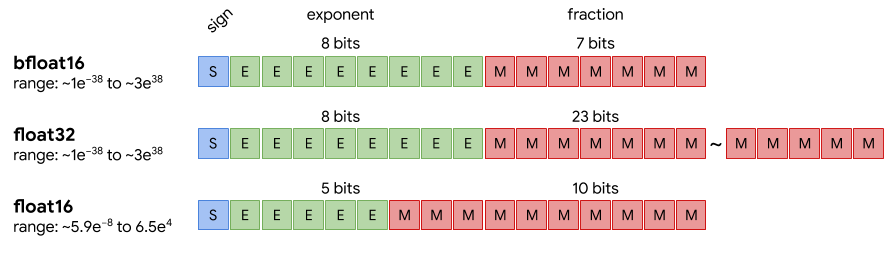
\includegraphics[width=\textwidth]{bfloat16.png}
	\caption{Representation of the bfloat16 format. (Taken from~\cite{bfloat16})}
	\label{fig:bfloat16}
\end{figure}
By using the exponent lenght the float32, the blfoat16 allows a quick conversion
data type conversion by dropping, or adding, the extra bits between float32 and bfloat16.
Moreover, with a smaller mantissa size, the hardware chips for the blfoat16 multiplier
is about half the size as the ones for float16 and around 8 times smaller than for float32~\cite{bfloat16}.
Moreover, since Neural Networks (NNs) are far more sensitive to the exponent range than the mantissa,
the blfoat16 performs really as it keeps the exponent range from float32.

Outside of standard Deep Learning frameworks, a variety of different data type were
studied to reduce the precision of machine learning models.
The work from~\cite{Johnson2018-up} evaluates a new \textit{posit tapered} data 
format which combines idea from posit~\cite{Gustafson2017-wo} format and log number system.
Various other studies use different custom floating point formats with reduced 
exponent and mantissa size~\cite{Lesser2011-mn, Chen2018-an, Vicuna2021-mw, Wang2018-oo}.
The authors in~\cite{Carmichael2019-nu} design three FPGAs for low-precision fixed
point, floating point, and posit.

\section{Implementing reduced precision}
To remain efficient, consumer hardwares only support a limited set of data formats; for exmaple IEEE~754.
The use of custom data format often requires either: specialized hardware, software implementation, or simulation.

With comodity hardware only supporting the most popular data formats, implementing a new format can be tricky.
A straight forward way to achieve this is to design a custom specialized hardware capable of executing the new format.
The authors in~\cite{Carmichael2019-nu} designed three different FPGAs to support low-precision floats, fixed points, and posits.
Another study~\cite{Johnson2018-up} designed a \SI{28}{\nano\meter} ASIC implement an 8-bit Exact Multiply-Accumulator (EMAC).
On the one hand, the key advantage of designing specilaized hardware is efficiency.
Indeed FPGAs and ASICs, designed for a single tasks can be optimize muc more than a general purpose hardware.
Major hardware manufacturers such as Nvidia and Google design specialized hardware
for frequent Deep Learning tasks (GEMMs), respectively with their recent GPU architectures and TPUs~\cite{tpu}.
On the other hand, creating new hardware is costly both in time and material.
This is especially true when performing study that evaluate a range of different data formats.

Since hardware implementations can be challenging to implement, some research investigated
software solution to implement reduced precision.
In~\cite{Anderson2016-yn}, the authors proposed a new data format, \textit{flyte},
with a mantissa that differs in 8-bits increment from the traditional IEEE~754 
standard while keeping the exponent the same.
This allows the use of native instruction to read data with power-of-two bit width.
To prevent cache miss due to misaligment, the authors suggest a packing and shuffling
method to reorganize the flyte in the vector registers.
However, for some flyte format, there are still some issue with misaligment resulting
in lower performance gain.
Overall, their technique show significant reduction in cache miss for \textit{BLAS}
Level 2 and 3; as many as $4.5\times$ less than with double.
The authors in~\cite{Zucker1994-rg} propose an algebraic method to pack multiple
low-precision operations into a single high-register operation.
This method showed performance improvement of 8.7\%, 13.6\%, and 16.2\% when packing
2, 4, and 8 number respectively.
Unfortunately, this technique can only be applied to a few algebraic operations.
On the one hand, software implementations are not as efficient as specialized hardware
since they suffer from substantial overhead cost.
Implementing software solution often requires high manual efforts whether to  perform
code conversion or to design a new data format.
On the other hand, software design have the potential to be more portable accross
architecture compared to specialized hardware.

As an alternative to hardware or software implementation, a common approach to 
prototype or do studies of new data format is through simulation.
The authors in~\cite{Chatelain2019-fu} explore the use of reduced precision to 
lower communication cost of iterative methods.
They use the VPREC backend in verificarlo to simulate reduce precision combined
with an heuristic to determine a minimum precision for the different iterations.
Both temporal and spatial change in the precision of applications are considered.
Other studies~\cite{Higham2019-yd,Zhang2019-xv} propose simulation methods for reduced
precision on single operations and on kernels.
\textit{Highman et al.} implemented a reduced precision library in MATLAB while 
\textit{Zhang et al.} developed a high-level framework on top of PyTorch to use
reduced precision techniques.
The main benefits of simulating reduced precision is the low implementation cost 
and new hardware does not need to be designed.
This often allows to explore a large number of data format for a with less efforts.
Unfortunately, while simulation is great for accuracy, it is still challenging to 
simulate performance due to the complexity of modern system.
Moreover, simulating reduced precision comes at a substantial overhead cost.
Therefore, it is required to implement an hardware or software implementation later on to achieve performance.

\section{Quantization in Deep Learning}
In recent years, machine learning, and more specifically Deep Neural Networks (DNNs),
have seen a rise in popularity due to their ability to solve challenging problems.
However, the complexity of DNNs models come with high usage of computing resources.
With the enormous dataset required to train these models, a usual bottleneck is with compute and data communication time.
This motivated multiple studies \cite{Johnson2018-up,Wang2018-oo,Lesser2011-mn,Chen2018-an,Judd2015-kw,Vicuna2021-mw}
to explore the possibility of reducing the precision for the data format used to train those models.
This section explores the quantization methods developed in the Deep Learning 
domain to reduce the compute and data communication of models.

The authors from multiple studies explored the effects of quatization for SVM classification
and found that it is possible to use minimal precision without accuracy loss.
In~\cite{Lesser2011-mn}, the authors investigate the impacts of reducing precision for SVM
classification and estimate the minimal precision required to achieve classification 
without loss of accuracy. Three experiments are performed: 
(1) adding noise to parameters,
(2) using MPFR, simulating reduced mantissa precision from 53 to 4 bits,
and (3) combining the experiment (1) and (2) concurrently.
By comparing the effects of quantization with and without rounding, it is possible To
better isolate the impact of rounding due to reduced precision.
The authors benchmark their experiments on three datasets: SONAR, IRIS, and MUSK.
They use the double precision results as a reference for the classication error.
The results show that lowering the precision up to 15 bits does not affect teh accuracy
for classificatio; this is consistent with the literature.
Further understanding the bounds for reducing the precision would allow to automatically
adjust the precision for classification, which would be an effort towards addressing the third 
challenge from Section~\ref{sc:rp-problem-definiton}.

With DNNs becoming more complex it becomes difficult to train the models with using 
techniques to improve performance such as data sampling or model parrallelism.
It is also problematic to integrate those models on embedded systems due to resource limitations.
While many study found that CNNs are resilient to accuracy loss when using reduced precision,
few of them attempted to vary the precision used at each layer.
The authors in~\cite{Judd2015-kw} show that the precision required in different layers and networks
differs significantly.
Moreover, they suggest a method to select the appropritae precision of each layer while 
keeping accuracy within a determined boundary.
Their model conver floating-points to the appropriate representation then back to single-precision after processing a layer.
To evaluate their method, the authors benchmark their reduced precision model on 5 popular CNNs.
Through their experiments they reduce the precision of both the weight of the model and the output of each layer.
Their first experiment reduced the precision of all layer simultaneously in the range of 12 to 1 bits.
The results show that only 21 bits would be required to store both the weight and output data of a layer.
The authors proceed by reducing the precision of each layer one by one to obtain an idea of the importance of precision for all layers.
From the results, we observe that the precision required by each layer varies significantly.
The authors also calculate an estimate data communication for the networks.
They also propose a method to find the minimal precision per layer while preserving accuracy:
\begin{itemize}
	\item[1.] Set the layers to an initial uniform precision with less than $0.1\%$ error.
	\item[2.] Create a collection of deltas by reducing the precision of parameters and layer output by 1 bit for each layer.
	\item[3.] Use the configuration giving teh best accuracy for the next iteration.
\end{itemize}
To find the \textit{best}, although potentially sub-optimal, the authors use a Pareto
frontier between the amount of data transfer and the accuracy for different configuration of bit precision.
Although sub-optimal, this heuristic resulted in a average decreas of $74\%$ of data traffic
while preserving accuracy within $1\%$ of tolerance.
This work show the potential of using various precision size for different layers of CNNs.
It motivates further efforts to study strategies in further exploiting reduced precision
to reduce memory usage and compute time. 

Linear algebra operations are a critical components in most DNNs models such as 
the multiply-accumulate (MAC) operation; e.g.~$\sum_{i}a_{i}b_{i}$.
The authors in~\cite{Johnson2018-up} describe \textit{ELMA}, a new methods to compute MAC using a combination of logarithmic 
number system~(LNS), \textit{Kulisch accumulator}~(EMA), and the posit data format~\cite{Gustafson2017-wo}.
The authors evaluate the accuracy using an FPGA implementation of the ResNet-50~ImageNet model.
Moreover, the new ELMA implementation is compared in term of area~($\SI{}{\micro\metre}^2$)
and power~(\SI{}{\micro\watt}) using a \SI{28}{\milli\metre} ASIC library.
The results show that the proposed ELMA operator reduces the power usage on 
multiplications by \SI{90.9}{\micro\watt} but increase it for additions by \SI{68.3}{\micro\watt}.
Overall, the net power usage is lower than previous methods.
This suggest that further efforts to reduce floating-point efficiency could bring substantial benefits.

Without doubt, DNNs emerged as a powerful tool to solve problems.
However, to achieve high accuracy, DNNs require tremendous amount of resources;
with models reaching 100s of \SI{}{\mega\byte}s and computation on large datasets can span multiple days/weeks.
Moreover, data communication between learners is often another source of bottleneck during training.
Traditionally, applications are developed to be exact although it is not necessary for most tupes of data.
In~\cite{Chen2018-an}, the authors explore approximate computing to reduce both 
computation and data communication, while preserving accurate results.
The authors quantize the weight and activation of the model from 16 to 2 bits.
To evalute the accuracy, the reduce precision model are bencmark on four popular DNNs: CIFAR10-CNN, AlexNet, ResNet18, and ResNet50.
They find that at 4 bits the accuracy remains within $<1\%$ of the reference 
full-precision model while improving performance by $4.5\times$.
When reducing the precision of the models to 2 bits, the authors achieve a $14\times$
improvement in normalized chip density; resulting in lower energy comsumption.
Overall, the results from this paper show promising benefits to further study reduced 
precision strategies as it jointly reduces hardware and energy cost as well as compute and data communication time.

Numerous approximate computing methods have been studied for the field of deep 
learning to reduce computation and data communication time, and energy cost.
With the energy efficientcy of hardware increasing quadratically witht the reduction in bit precision.
With current hardware implementing 16 bit precision, we can see performance improvement of $\ge 4\times$ compared to 32 bits.
Studies showed that the computation steps for DNNs inference can be reduced to as low as 2-4 bits
while remaining accurate; and even precision of 1-2 bits for weights and activations.
However, an empirical study found taht precision of 16 bits was required during 
DNNs training to preserve accuracy.
When trying to reduce the precision even more, DNNs ofen start to see significant 
accuracy degradation, issues with convergence, and impac on overall accuracy.
The authors in~\cite{Wang2018-oo} suggest using \textit{FP8} combined with 
\textit{chunk-based computations} and \textit{stochastic rounding} to further reduce
the bit precision compared to state-of-the-art methods while maintaining accuracy.
They evaluate their methods on a collection of 6 NNs models accross multiple datasets.
The results depict that their implementation using both FP8 and FP16 is equivalent
in accuracy to using FP16 and FP32, while performing $2-4\times$ faster.
Moreover, the authors found that keeping a higher accuracy (FP16) on the first layer~(input data)
and the last layer was critical to successfully train their FP8 models.
This work shows that effort in reducing floating-point precision in deep learning
can increase performance significantly while keeping accuracy equivalent.

While machine learning model are a great tool to solve problems, they can be challenging
to implement on embedded systems due to their large memory requirement.
Mondrian Forest, a common online classifying algorithm, is typically too memory intensive
for embedded devices, therefore, using reduced precision could enable its use.
The authors in~\cite{Vicuna2021-mw} explore reduced precision techniques on Mondrian Forests
to reduce their memory usage.
They study the model parameters, numerical precision, and memory consumption together
due to their interdependence.
Using VPREC, the authors simulated reduced the bit precision $p$ in the range from 52 to 1 bits.
Moreover, the exponent range is varied from 11 to 2 bits.
To simulate the different memory requirements at different precision.
The model is instrumented both at a node level and for the whole model.
To evaluate their method, they use two publicly available dataset: Recofit, and Banos et al.
To quantify the performance of the model with different memory constraint, the authors allocate three
different values memory limit for the model: \SI{0.6}{\mega\byte}, \SI{1.2}{\mega\byte}, and \SI{3}{\mega\byte}.
Their results for node instrumentation show that for $p \ge 2$ the F1 scores remain with a standard deviation.
For the whole instrumenation, the F1 scores are significant different when $p \le 6$.
The observations on the F1 scores for $p > 2$ were not correlated to memory.
This suggest that using reduced precision with different memory allocation would yield similar results.
Given constant memory constraints, the authors found that using reduced precision allows the 
trees to grow deeper; potentially improving the classification performance.
Overall, the results show that Mondrian Forest can be implement with low-precision floating-points
of only 8 bits without affecting the F1 scores significantly.
This has the potential to reduce memory footprint by roughly $1.8\times$ compared to double precision.

Although Section~\ref{sc:rp-data-format} discussed the use of reduced and mixed precision
in popular deep learning framework like PyTorch and Tensorflow, the scope of ultra low 
precision (i.e. $\le 8$ bits) is still a topic limited to academia.
Further efforts is required to better understand the effects of reduced precision
on different models and datasets; without which, it the reach of ultra-low floating-point
will remain restrained.
While the deep learning community as vastly explored reduced precision techniques,
to the best of our knowledge, the topic remains unexplored in most other fields of application.

\section{Discussion}
In this chapter, multiple studies showed promising reduced precision approaches
to improve the performance of applications while preserving accuracy.
However, reduced precision comes with its own caveats.
Throught this section, we will discuss the different benefits and limitations from
using reduced precision.
Moreover, we will discuss open problems in the field of reduced precision.

By reducing the number of bits used to represent numbers, the memory footprint
of applications is directly reduced.
This has two main benifits: applications require less resources to execute, and 
it reduce the hardware cache miss therefore increasing performance.
Additionally, reducing the size of data format allows the use of specialized hardware
or software techniques to pipeline operations together.
With hardware complexity being approximately proportional to the square of the 
number of bits~\cite{Chen2018-an}, reducing the data format can jointly increase
performance and reduce energy cost.
Fusing multiple low-precision data format operations in a single register operation 
has the potential to lower computational cost substantially.
Lastly, reducing the size of input and output data would let to lower storage space requirements.

To make use of reduced precision, substantial efforts is required in creating, 
evaluating, and implementing new data formats.
% TODO
% Change sentence to reflect that its really for the interaction between precision and the application.
% That is what precision is needed for a specific application.
This is amplified by the current lack of understanding in the 
behavior of different application using reduced precision.
Even within a single application, varying the data can substantially modify the 
precision required to preserve accurate results.
Therefore, designing new hardware and software solutions incurs a high cost in manual effort.
Moreover, while using a lower-precision data format on an application might yield 
promising results, changing the data used could lead to unpredictable accuracy changes.
Finally, the conversion between data formats comes with an overhead cost.
Thus, attention needs to be paid to minimize the amount of data format conversions 
within an application, when applying reduced precision.
Otherwise, the performance benefits from using reduce precision might be overtaken
by a high overhead cost in data conversion and result in an overall slowdown 
the perfomance of an application.
% TODO
% Discuss in brief the different type of implementation for reduced precision.

To have a broader adoption of reduced precision some critical limitations need to 
be addressed, including but not limited to:
\begin{itemize}
	\item Determine the different sections of code that can take advantage of reduce precision 
	      while considering both temporal and spatial variability of precision.
	\item Improve the heuristics for finding the minimal precision required for each code section.
	\item Estimate the perfomance gain from using reduce precision.
	\item Understand the effects of reduce precision when varying the data in an application.
	\item Automate the code conversion to simplify the usage of reduce precision.
\end{itemize}
To the best of our knowledge, these problem remains open challenges within the field of reduce precision.
Furthers research will be needed to make progress on resolving these challenges.
